\documentclass[11pt,a4paper]{article}
\usepackage[margin=24mm]{geometry}
\usepackage[T1]{fontenc}
\usepackage{lmodern,microtype}
\usepackage{graphicx,booktabs,longtable,tabularx,array,amsmath,amssymb,xcolor,enumitem,listings,fancyhdr,float}
\usepackage[colorlinks=true,linkcolor=teal,urlcolor=teal,citecolor=teal,breaklinks=true]{hyperref}
\setlength{\parindent}{0pt}
\setlength{\parskip}{6pt}
\setlength{\emergencystretch}{3em}
\setcounter{tocdepth}{2}
\pagestyle{fancy}\fancyhf{}\fancyhead[L]{ASDMotion: data-first research dossier}\fancyhead[R]{16 September 2026}\fancyfoot[C]{\thepage}
\setlength{\headheight}{14pt}
\newcolumntype{P}[1]{>{\raggedright\arraybackslash}p{#1}}
\newcommand{\artifact}[1]{\nolinkurl{#1}}
\title{Understanding ASDMotion Before Choosing a Model\\\large Data, algorithms, reproducibility, and research directions}
\author{Research workspace dossier}
\date{16 September 2026\\Version 1.0 --- measured release audit and scoped literature search}
\begin{document}
\maketitle
\begin{abstract}
This dossier starts from the public Dinstein-Lab repository, the released skeleton data, and the 2024 JAMA Network Open paper. The central finding is a mismatch between the current labeled release and the published experiment, including a strong association between frame rate and label and substantial missing-pose imbalance. These are measured release properties, not proof that the published experiment was invalid. The most defensible first research objective is to establish movement recognition that survives these data-quality and acquisition checks. The document distinguishes source claims, code observations, measured data properties, and new research proposals. It provides a phase-by-phase plan and executable analysis code, followed by recent studies that ask different questions about autism and motion.
\end{abstract}
\textbf{Read first:} Sections~\ref{sec:findings} and \ref{sec:data} describe what was actually downloaded and measured. Then read the original-paper explanation, code audit, representation tutorial, and research plan. The source paper remains the authority for its claims; this report is a research analysis, not a clinical assessment.
\begingroup\small\tableofcontents\endgroup
\clearpage
\section{Findings that determine the research strategy}\label{sec:findings}
\begin{enumerate}[leftmargin=*]
\item \textbf{The target is movement measurement within an ASD cohort.} Stereotypical motor movement (SMM) is one aspect of restricted/repetitive behavior. The study has no non-ASD diagnostic comparison group. A negative movement clip does not mean a non-autistic child. \cite{barami2024}
\item \textbf{The downloaded labeled release differs from the paper.} It contains 36,930 records, 8,267 positives and 28,663 negatives. The publication describes 36,000 selected segments, including 7,352 positives. The release has 329 distinct first identifier tokens; these are not verified participant IDs. Results below refer to the files hashed in \artifact{data/raw/manifest.json}, not automatically to the paper's cohort.
\item \textbf{Acquisition metadata alone separates many labels.} All 28,663 negatives have 25-fps metadata; 6,520 positives have 30-fps metadata. A post-hoc rule declaring every 30-fps clip positive has precision 1.000 and recall 0.789 on this release without examining movement. This is a dataset diagnostic, not a validated predictive model. \artifact{data/processed/shortcut_audit.json}.
\item \textbf{Missingness is informative about labels.} There are 3,276 completely zero-pose clips: 3,264 negative and 12 positive. At clip level, the average fraction of zero-confidence joints is 40.89\%. Zero coordinates must not silently become a real body location or a stationary child. \artifact{data/processed/dataset_summary.json}.
\item \textbf{Evaluation setting changes the interpretation.} The paper's initial continuous-test frame precision/recall are 36.64\%/87.72\%. The headline 66.82\%/92.53\% uses selected reannotated segments. These are different reference-label/evaluation settings. \cite[pp.~5--8]{barami2024}
\item \textbf{The public implementation needs repair before end-to-end reproduction.} Counterexample tests demonstrate fresh-input failures, event-merging defects and denominator risks. Source findings are pinned to repository snapshots; they do not establish which historical code ran the published experiment. \artifact{reports/pipeline_audit.md}.
\item \textbf{Recent work broadens the question beyond classification.} Relevant perspectives include repetition topology, concurrent movement labels, fine hand kinematics, interpersonal synchrony, neural--motor coupling and measurement validity. This search did not verify independent reuse of these released ASDPose files; citing the paper is not evidence of reuse. Section~\ref{sec:literature} gives sources and scope.
\end{enumerate}

\section{The downloaded data: measured release properties}\label{sec:data}
\subsection{Keep the acquisition levels separate}
A child can contribute several assessments; an assessment can have several synchronized cameras; one camera stream can yield many overlapping or selected clips; a clip has many frames; each frame has joints. These levels are not interchangeable sample sizes. The paper's 580 hours are camera footage, not 580 hours of unique independent participant time. A valid subject-disjoint design must keep every view and repeated session from a child in the same partition. \cite[pp.~3--4]{barami2024}

\subsection{Files and what they can support}
\begin{tabularx}{\linewidth}{@{}l r X@{}}\toprule
Artifact & Bytes & Interpretation\\\midrule
\artifact{dataset.pkl} & 5,094,311,994 & Labeled selected skeleton clips; all records profiled.\\
\artifact{asdpose.zip} & 7,846,880,820 & Separate skeleton archive advertised without annotations; inventory retained separately.\\
\artifact{model.pth} & 24,235,571 & Released model checkpoint; downloaded, not executed.\\\bottomrule
\end{tabularx}
\par Sources: repository download links and \artifact{data/raw/manifest.json}. The original paper states raw identifiable videos are not publicly released; do not treat these skeleton files as RGB video access. \cite[p.~9]{barami2024}

\subsection{Continuous recordings: complete archive audit}
\label{sec:continuous-audit}
All 914 numeric pickle members of \artifact{data/raw/asdpose.zip} were
successfully decoded and profiled, one member at a time directly inside
the archive, with the restricted NumPy unpickler. No full extraction was
needed. The ZIP also contains \texttt{db.csv}; its extracted manifest has
914 rows, no duplicate filenames, and an exact one-to-one filename match
to the pickle members. Archive CRC validation passed separately.
These are measured local-release facts, reproducible with
\artifact{scripts/07_profile_continuous.py}; per-recording results are in
\artifact{data/processed/continuous_inventory.csv}, aggregate results in
\artifact{data/processed/continuous_summary.json}, and CRC/inventory
evidence in \artifact{data/processed/archive_summary.json}.

\begin{table}[htbp]
\centering\small
\begin{tabular}{P{0.42\linewidth}rr}
\toprule
Quantity & Downloaded archive & Paper \\
\midrule
Children, explicit manifest ID & 241 & 241 \\
Assessments, child/type/index combinations & 318 & 319 \\
ADOS assessments & 226 & 226 \\
PLS assessments & 70 & 71 \\
Cognitive assessments & 22 & 22 \\
Camera recordings & 914 & 883 \\
Camera-stream hours & 599.77 & approximately 580 \\
\bottomrule
\end{tabular}
\caption{Released continuous-archive inventory compared with paper
denominators. Archive hours are $\sum T/\mathrm{fps}$; declared metadata
duration sums to 599.75 hours. Simultaneous camera views contribute
separately, so these are not unique child-observation hours.
Paper values: \cite[pp.~3--4]{barami2024}.}
\end{table}

The manifest explicitly identifies \texttt{child\_id}, assessment type,
\texttt{assessment\_index}, \texttt{camera\_index}, and filename.
This is stronger identity evidence than parsing anonymous labeled-clip
prefixes. However, the mapping between annotated-release identifiers and
these manifest identities has \textbf{not been verified}. The release
differences above must not be silently harmonized, and clinical metadata
must not be joined to annotated clips using an assumed numeric-ID match.
The continuous files contain poses and detection metadata; these
inventories do not provide a verified continuous event-label crosswalk.
Evidence: \artifact{data/interim/archive_metadata.csv},
\artifact{data/processed/dataset_structure.json}, and
\artifact{data/processed/continuous_summary.json}.

Every continuous member has one person slot, 17 joints, two coordinate
channels, and \texttt{float64} coordinates: $[1,T,17,2]$; confidence has
shape $[1,T,17]$. Across the archive there are 62,698,358 pose frames.
The median stream duration is 2,138.80 seconds (35.65 minutes), ranging
from 449.44 to 5,398.12 seconds. Stored frame rates range from 21.694899
to 30.300812 fps and frequently have fractional values. Rounded to the
nearest integer, 679 files are 30 fps, 234 are 25 fps, and one is 22 fps;
these rounded groups are descriptive, not resampling instructions.
Several original image-shape tuples occur, including both landscape-like
and portrait-like orderings. Establish the shape convention from provenance
before feeding them into a model. Evidence:
\artifact{data/processed/continuous_inventory.csv} and
\artifact{data/processed/continuous_summary.json}.

\paragraph{Missingness is substantial in the full recordings.}
Exactly 20,178,332 frames (32.18\% of all pose frames) have all-zero
coordinates, and the aggregate all-zero-confidence-frame count is the
same. Two entire recordings have all-zero poses. The median recording has
28.60\% all-zero pose frames, with an interquartile range of
15.55--48.19\%. Zero-valued pose frames represent unavailable signal in
this audit; the files alone do not establish whether the child was absent,
occluded, undetected, or lost during preprocessing. No nonfinite coordinate
or confidence values were found, but 176,069 confidence entries fall
outside $[0,1]$. Confidence should therefore be audited before treating it
as a bounded weight or probability. Per-joint mean confidence, including
missing zeros and weighted by available array entries, ranges from about
0.195 at the right ankle to 0.514 at the left shoulder; these differences
are not direct estimates of anatomical movement quality. Evidence:
\artifact{data/processed/continuous_summary.json}.

\paragraph{Frame-count metadata require explicit alignment.}
In 234 files, declared \texttt{frame\_count} differs from the pose-array
length $T$. In every profiled file the equality
\begin{equation}
 \texttt{frame\_count}-T=\texttt{adjust}
\end{equation}
holds; the observed adjustment ranges from $-163$ to $4$.
This establishes an accounting relation, not where in time frames were
added or removed. The largest difference between stored duration and
$T/\mathrm{fps}$ is 6.52 seconds. Annotation alignment must recover the
meaning and temporal location of these adjustments before evaluating
onset/offset accuracy. Evidence:
\artifact{data/processed/continuous_inventory.csv} and
\artifact{data/processed/continuous_summary.json}.


\subsection{A concrete record and its dictionary}
The top-level labeled pickle contains \artifact{annotations} and \artifact{split}; the latter maps \artifact{train}/\artifact{test} to sets of identifiers. The first record has coordinates of shape $(211,17,2)$, confidence of shape $(211,17)$, \artifact{fps}=30, \artifact{total_frames}=211, \artifact{action_name}=Clapping, \artifact{binary_label}=1, \artifact{start_frame}=649, \artifact{end_frame}=654 and identifier \artifact{1_1_1_Clapping_649_654}. Its coordinates are float64. There is no explicit person axis in these clip records. These observations are measured in \artifact{data/processed/dataset_structure.json}.

\begin{longtable}{@{}P{.24\linewidth}P{.31\linewidth}P{.38\linewidth}@{}}\toprule
Field & Meaning established by inspection & Caution for use\\\midrule\endhead
\artifact{keypoint} & Time $\times$ 17 joints $\times$ 2 coordinates & Pixel-like 2D positions; not anatomical 3D trajectories.\\
\artifact{keypoint_score} & Time $\times$ joint pose confidence & Zero dominates some clips; not an SMM probability.\\
\artifact{fps}, \artifact{total_frames} & Stored sampling rate and array length & Use actual stored fps for duration. All declared lengths match arrays.\\
\artifact{img_shape} & Stored pair of dimensions & Mixed values and orientation conventions; verify width/height before normalization.\\
\artifact{binary_label} & 0 matches NoAction; 1 denotes positive movement annotation & Not ASD/non-ASD status.\\
\artifact{action_name} & Single or comma-separated movement names & 1,572 clips contain combined labels; split strings for multilabel analysis.\\
\artifact{identifier} & Unique-looking concatenated tokens & Two repeated identifiers have different arrays. Prefix meanings are not documented in the file.\\
\artifact{start_frame}, \artifact{end_frame} & Numeric boundary metadata & Names do not establish units; the first difference is 5 while there are 211 frames.\\\bottomrule
\end{longtable}

\subsection{Counts and a reproducibility discrepancy}
The downloaded file has 36,930 clips: 8,267 positive (22.39\%) and 28,663 negative. The original paper reports 7,352 positives and 28,648 negatives. The current file is therefore not an exact count match to the reported experimental selection. This is evidence requiring version reconciliation, not evidence of a particular explanation. The public README added the annotated-file link in its 3 October 2025 commit. \cite{repo,barami2024}; local \artifact{dataset_summary.json}.

The release split contains 32,179 training records (7,210 positive) and 4,751 test records (1,057 positive). The training split set has 32,177 unique identifiers because two identifiers repeat among records. There are 289 and 40 distinct first identifier tokens respectively, with no overlap. Across all records, there are 329 first-token groups, 372 first-two-token groups and 1,116 first-three-token groups. These are \emph{candidate} subject/session/video groupings, not confirmed participant counts. The paper's 220/21-child split cannot be claimed from these observations. The release has no separate validation partition. \artifact{data/processed/released_split_audit.json}.

\subsection{Frame rate is a strong label-associated artifact}
\begin{table}[H]\centering
\begin{tabular}{@{}llrr@{}}\toprule
Split & fps & Negative & Positive\\\midrule
Train & 25 & 24,969 & 1,445\\
Train & 30 & 0 & 5,765\\
Test & 25 & 3,694 & 302\\
Test & 30 & 0 & 755\\\bottomrule
\end{tabular}
\caption{Measured metadata-label contingency, generated from every released clip. Source: \texttt{fps\_label\_crosstab.csv}.}
\end{table}
The metadata-only rule $\widehat y=\mathbb{1}[\mathrm{fps}=30]$ gives 100\% precision and 78.87\% recall over all released clips. This rule was chosen after inspecting the release; it is not a preregistered holdout result and must not be compared to the paper's frame-level performance. It proves that strong label separation is available without motion analysis. It does not prove that PoseC3D explicitly reads the fps field or learned this exact rule.

Possible mechanisms to investigate include different extraction paths, resampling, source subsets or changed release contents. These explanations remain unverified. Even if fps is omitted from model input, duration, sampling cadence, image geometry and missingness can retain acquisition information. Matching fps and preprocessing is a necessary diagnostic, not proof that all confounding has been removed. \artifact{scripts/04_shortcut_audit.py}.

\subsection{Missing poses and duplicates}
Completely zero coordinates and confidence occur in 3,276 clips: 3,264 negatives (11.39\% of negatives) and 12 positives (0.15\% of positives). Across clips, mean zero-confidence fraction is 0.4089 and mean fraction below an analyst-selected confidence threshold of 0.2 is 0.4613. The latter is not a calibrated measurement-error probability. Low-confidence estimates (score below 0.2) are disproportionately common at wrists, knees and ankles relative to shoulders.\par
The clip audit additionally found 49,851 confidence entries outside $[0,1]$, with no nonfinite confidence entries. As with the continuous archive, these stored scores should not be assumed bounded probabilities without checking their preprocessing history. All 36,930 original clip coordinate arrays have three dimensions, confirming the absence of a person axis in this labeled release.\par
Source: \artifact{data/processed/dataset_summary.json} and \artifact{quality_motion_by_label.csv}. These are descriptive release statistics, not estimates for the original clinical population.

There are 3,221 repeated coordinate arrays beyond their first occurrences. Forty-three coordinate hashes occur in both release partitions, but all cross-partition shared hashes are all-zero arrays; no nonzero coordinate hash crossed the split in this check. This must not be reported as proven duplicate real movements leaking across train/test. Bytewise duplicate checks do not detect near-duplicates, overlapping windows, alternate camera views or the same child under another identifier. The two duplicate identifier strings correspond to different coordinate hashes, so identifier-only deduplication would silently discard distinct records. \artifact{released_split_audit.json} and \artifact{exact_coordinate_duplicates.csv}.

\subsection{Timing, motion and labels}
Clip duration, computed as array length divided by stored fps, has median 12 seconds, interquartile range 8--17.04 seconds, minimum 2.96 seconds and maximum 285.04 seconds. Positive and negative medians differ: 8.04 versus 13.04 seconds. Summing clips gives 134.32 hours, \emph{not} unique continuous recording duration: overlap, resampling and repeated views may be present. \artifact{dataset_summary.json}, \artifact{quality_motion_by_label.csv}.

For 24,961 clips, duration minus $(\texttt{end\_frame}-\texttt{start\_frame})$ is exactly 2 seconds; another 9,416 yield 2.04 seconds and 2,184 yield about 2.033 seconds. One plausible interpretation is second-based event bounds with approximately one second of padding at each side, but this is an inference requiring producer confirmation. Do not multiply these fields by fps or use them as frame indices until their convention is established. \artifact{shortcut_audit.json}.

\begin{figure}[p]\centering
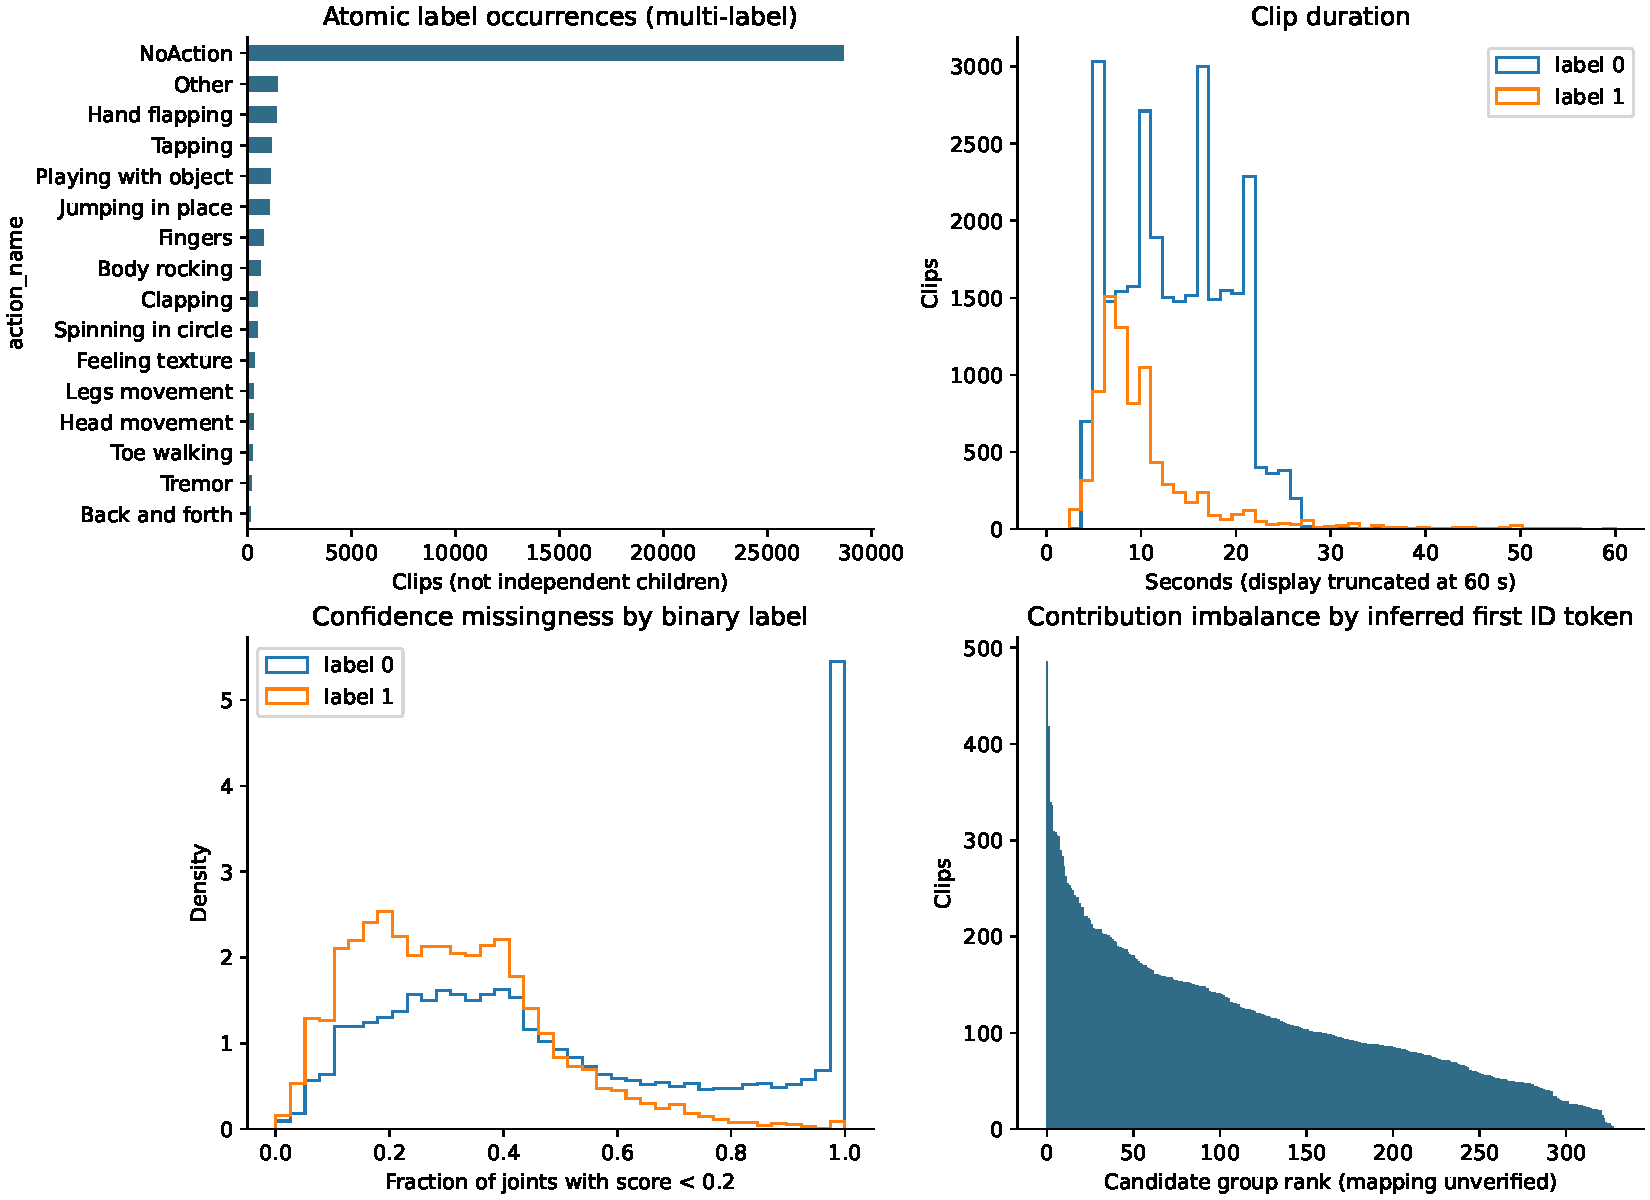
\includegraphics[width=\linewidth]{../../reports/figures/release_overview.pdf}
\caption{Measured release overview. Label counts count atomic names, so combined labels contribute to several categories. The grouping plot uses unverified identifier prefixes. The confidence threshold 0.2 is an audit choice. Duration display is truncated at 60 seconds.}
\end{figure}

\subsection{What is not established by the public clip file}
The inspected records do not contain age, sex, diagnostic scores, medication, individual clinical severity, intervention exposure, a verified participant crosswalk, annotator disagreement or explicit camera calibration. The original paper's cohort-level descriptive statistics cannot be assigned to individual records. Video context, facial expression, detailed finger articulation, sensory triggers and subjective function cannot be reconstructed from 17 body joints. Some of these questions may become possible with additional authorized data, but they are not current measurements. The need for an author-supplied version/split/timing explanation is recorded in \artifact{docs/OPEN_QUESTIONS.md}.

\clearpage
\section{What the original paper establishes}
\label{sec:original-paper}

This section describes the publication. The current release must not be assumed identical to its experimental dataset: the separate data audit in this report identifies different clip counts, mixed frame rates and missing-pose patterns. Publication claims and measured release properties remain separate until their versions are reconciled.

\subsection{The target is SMM measurement within ASD}
Barami and colleagues introduced ASDMotion, an algorithm for detecting stereotypical motor movements (SMMs), and ASDPose, the associated skeletal-motion dataset. SMMs include hand flapping, rocking, jumping and other repetitive movements. They are one aspect of restricted and repetitive behaviour, not a complete description of autism spectrum disorder (ASD). The paper explicitly notes that SMMs are neither universal in ASD nor exclusive to ASD and can have a self-regulatory function. Consequently, this study supports measurement of movement in children already diagnosed with ASD; it does not establish an ASD diagnostic classifier, a movement's psychological function, or whether that movement should be reduced. \cite[pp.~1--3]{barami2024}

\subsection{Cohort, acquisition hierarchy, and selection}
The study selected children with a DSM-5 ASD diagnosis and an ADOS-2 score of at least 2 on item D2 or the relevant D4/D5 stereotypical-behaviour item. Participants were recruited in 2017--2021 through the Azrieli National Centre for Autism and Neurodevelopment Research, connecting Ben-Gurion University with eight clinical sites. The age range was 1.4--8.0 years. This is a cohort selected for repetitive behaviour, not an unselected screening population. \cite[p.~3]{barami2024}

The reported acquisition hierarchy is:
\[
241\ \text{children}\ \longrightarrow\ 319\ \text{assessments}
\ \longrightarrow\ 883\ \text{camera recordings}
\ \longrightarrow\ 580\ \text{camera-hours}.
\]
Each child contributed one or two assessments; two to four cameras recorded each assessment at 30 frames/s and $1080\times1920$ resolution. Assessment types were 226 ADOS-2, 71 PLS-4 language assessments, and 22 cognitive/developmental assessments (11 Mullen and 11 WPPSI-III). Simultaneous views therefore do not represent additional independent child-observation time. Clips, views and repeated assessments are nested within children. \cite[p.~3]{barami2024}

The recognition training group comprised 220 children/295 assessments; the test group comprised 21 children/24 assessments. Training demographics were 172 males, 48 females and mean age 3.97 years (SD 1.30); test demographics were 15 males, 6 females and mean age 4.32 (SD 1.39). The abstract's 172 males and age 3.97 reproduce the training entries even though the sentence refers to the entire cohort. These should not be repeated as pooled cohort statistics. \cite[pp.~1,4]{barami2024}

\subsection{Pipeline: representation and the reason for each stage}
\begin{enumerate}[leftmargin=*]
\item \textbf{Extract pose.} OpenPose estimates 17 body-joint locations in two image dimensions for every person in every frame. This compresses the raw image into body geometry while retaining motion across frames. The paper does not release the raw RGB videos. \cite[pp.~3,9]{barami2024}
\item \textbf{Track identities.} An off-the-shelf spatiotemporal-affinity-field method keeps skeleton identities consistent across frames, supporting annotation and person selection. It was not additionally trained on this cohort. \cite[p.~3]{barami2024}
\item \textbf{Select the child.} A COCO-pretrained YOLOv5 was trained on 30,000 frames from annotated positive segments, using an 80/20 split. Reported child-box precision and recall were 95\% and 92\%. The main text does not establish a child-disjoint split for this separate detector. Skeleton and YOLO boxes are matched by intersection-over-union; unmatched skeletons become adult, while unmatched detection boxes are discarded. Errors here can remove the target before motion classification. \cite[pp.~3--4]{barami2024}; Supplement~1, p.~3.
\item \textbf{Construct positive/negative clips.} Annotators reviewed 580 hours and marked 7,352 positive segments, with event boundaries, movement type and child identity. The authors sampled 28,648 negatives with a matching length distribution. Training contained 6,597 positives and 24,923 negatives. The test cohort contained the remaining 755 positives. These are paper-reported counts, distinct from any independently inventoried release files. \cite[pp.~3--4]{barami2024}
\item \textbf{Recognise motion.} PoseConv3D pretrained on Kinetics-400 operates on joint-confidence heatmaps. A training sample spans 200 original frames (about 6.7 seconds), while its model representation uses 48 two-dimensional heatmaps. Three-dimensional convolution learns across two spatial axes and time; this is not a measured three-dimensional skeleton. The supplement reports batch size 64, stochastic gradient descent and 100 epochs, at 83.49 minutes per epoch for the chosen model. Exact sampling and augmentation must be checked in code. \cite[p.~4]{barami2024}; Supplement~1, pp.~7--8.
\item \textbf{Scan long recordings.} At inference, 200-frame windows advance by 30 frames; a frame receives the maximum score of all covering windows. Thresholding and joining contiguous positives yields detected episodes and assessment summaries. \cite[pp.~4--5]{barami2024}
\end{enumerate}

The 13 manually annotated movement categories include gross-body movements, finger flicking and repetitive object play, but the trained label is binary: any SMM versus non-SMM. The supplement states explicitly that categories were pooled. A methodological implication is that fine-finger and object-context information may be only partially represented by a coarse body skeleton; the paper does not experimentally quantify that information loss. (Supplement~1, pp.~5--6.)

\subsection{Mathematical view of the temporal decision}
The following notation explains the paper's verbal procedure; it is not an equation reproduced from the article. Let $t$ be a frame index, $W_k$ the frames covered by window $k$, $s_k\in[0,1]$ its score, $q_t$ the merged score, $\tau$ the threshold and $\widehat y_t$ the predicted binary label. The indicator $\mathbf{1}[A]$ equals one when condition $A$ holds:
\[
q_t=\max_{k:t\in W_k}s_k,
\qquad \widehat y_t=\mathbf{1}[q_t\geq\tau],
\qquad \tau=0.85.
\]
The paper calls 0.85 an arbitrary threshold and examines values from 0.5 to 0.9. Consecutive positive frames are joined into events. Missing-pose handling, last-window handling and frames lacking valid windows are implementation questions, not specified by this equation. \cite[pp.~4--5]{barami2024}

For a specified population of evaluated frames, let $TP$, $FP$, $FN$ and $TN$ count true positives, false positives, false negatives and true negatives. Then the reported metric terminology corresponds to
\[
\mathrm{Precision}=\frac{TP}{TP+FP},\quad
\mathrm{Recall}=\frac{TP}{TP+FN},\quad
\mathrm{Specificity}=\frac{TN}{TN+FP},\quad
\mathrm{NPV}=\frac{TN}{TN+FN}.
\]
The evaluation population and aggregation weights matter as much as these formulas. The original continuous evaluation and the selected reannotation experiment below are different populations. \cite[pp.~5,7]{barami2024}

\subsection{Two evaluation stages that must remain distinct}
\paragraph{Initial continuous evaluation.}
On the original annotation of the held-out 24 assessments from 21 children, frame-level precision was 36.64\% (95\% CI 29.97--49.99\%) and recall was 87.72\% (84.22--94.22\%) at threshold 0.85. These results describe high recall with many apparent false positives. The sex-specific comparison involved 15 male and six female children; lack of a significant difference does not demonstrate subgroup equivalence. \cite[p.~5]{barami2024}

\paragraph{Selected reannotation experiment.}
The authors extracted 1,456 short segments with equal counts from the original true-positive, false-positive, true-negative and false-negative strata. Two annotators, blinded to model and original labels, judged the segments independently; agreement was 90\% and Cohen's $\kappa=0.76$. A segment was relabelled positive if either annotator called it positive. Reinspection converted 51\% of apparent false-positive segments into true positives and 9.8\% of false negatives into true negatives. \cite[pp.~5--7]{barami2024}

This experiment produced the headline precision 66.82\% (95\% CI 55.28--72.05\%) and recall 92.53\% (81.09--95.10\%), with specificity 95.45\% and NPV 99\%. These are not event-detection accuracy or ASD diagnostic accuracy. The paper describes reinspection of selected segments, not independent exhaustive reannotation of every frame of the continuous test set. Sampling equally from original error strata changes the reviewed composition; the exact weights and effective denominators behind the final summary percentages cannot be reconstructed from the published values alone. \cite[p.~7]{barami2024}

\paragraph{Assessment-level quantification.}
Using reannotated data, the count/rate measure correlated with manual annotation at Pearson $r=0.80$ and concordance correlation 0.70. Percentage of time with SMMs had Pearson $r=0.88$ and concordance 0.73. Figure~3 plots SMMs per minute and time percentage per assessment; its 24 assessment observations should not be treated as 241 independent child-level validations. Correlation indicates association, while concordance also addresses agreement; neither establishes sensitive measurement of longitudinal clinical change. \cite[pp.~7--8]{barami2024}

\subsection{Model comparison and reported limits}
The supplement compares pretrained PoseC3D against unpretrained PoseC3D, ST-GCN and two-stream adaptive GCN. The selected pretrained model had the best reported precision and recall and the highest training time. ST-GCN encodes joints as graph nodes with spatial and temporal edges; the two-stream method separately models joints and bones. The same held-out cohort was used in this comparison and model selection. This supports the published choice under that protocol, but future experiments need a separate validation process and untouched final test data. (Supplement~1, pp.~7--8.)

The authors identify uncertain generalisation to other contexts, older children, non-ASD populations and other developmental conditions; limited female representation; lack of subtype classification; untested event onset/offset accuracy; and the need for richer intensity/severity measures. Storage, computation and video privacy are additional constraints. These are limitations and open tasks, rather than measured performance on those external populations. \cite[p.~9]{barami2024}

\subsection{Source consistency register}
\begin{itemize}[leftmargin=*]
\item The demographic table implies 187 males in the full cohort by addition, whereas the abstract reports the training count of 172. Training females are printed as 48 (22.82\%), but $48/220=21.82\%$. Prefer the source counts and split-specific ages until participant-level metadata is reconciled. \cite[pp.~1,4]{barami2024}
\item Cognitive scores are listed for $183+16$ children, with $t$-test degrees of freedom 214; language scores for $148+9$, with degrees of freedom 174. These do not match ordinary two-group tests on exactly the stated counts. Do not infer missingness from the test statistics. \cite[p.~4]{barami2024}
\item The stated $7{,}352\times9.89$ seconds gives approximately 20.20 hours, not the stated 21.14 positive hours. Rounding of the printed mean alone does not explain this; view/count conventions or a reporting error remain unresolved. \cite[p.~3]{barami2024}
\item Main-text medians are 0.12 SMMs/minute and 1.55\% time, whereas Supplement~1 eTable~2 gives 0.1 and 1.4\%. Assessment-level versus video-level aggregation may account for this, but the source does not explicitly reconcile them. Keep both denominators visible. \cite[p.~5]{barami2024}; Supplement~1, p.~7.
\item The main-text Kinetics-400 citation points to reference 43, which is actually the self-stimulatory-behaviour dataset; the supplement supplies the Kinetics reference. Bibliographic cross-references should be verified rather than copied mechanically. \cite[pp.~4,12]{barami2024}; Supplement~1, p.~9.
\end{itemize}

The detailed Markdown companion records exact page references, original figure/table page images, and the supplementary-file acquisition route. No original table or figure was redrawn. Supplement PDFs were retrieved from the official Europe PMC supplementary archive after the direct PMC links served browser-check HTML; the stored files were verified as readable PDFs.

\clearpage
\section{The data pipeline: representation, algorithm, and failure modes}
\label{sec:pipeline-audit}

\subsection{Evidence and scope}
This section audits the retrieved ASDMotion source at commit
\texttt{f699dc7} and its MMAction2 fork at \texttt{f632b7e}.
These are retrieved repository versions, not verified paper-era execution
versions. Source snapshots and full line-level evidence are preserved in
\texttt{references/source\_snapshots/} and
\texttt{reports/pipeline\_audit.md}. Ten executable counterexample tests
in \texttt{tests/test\_upstream\_semantics.py} pass; they reproduce the
documented upstream behaviors without CUDA or MMCV. A passing
counterexample test does not mean that the underlying behavior is correct.
No claim of reproduced training or published accuracy is made here.
The source references are the
\href{https://github.com/Dinstein-Lab/ASDMotion/tree/f699dc7b7af5726df5d8e79161d192eac22cfafb}{pinned ASDMotion repository}
and the
\href{https://github.com/TalBarami/mmaction2/tree/f632b7e56291805ac6d4debc8c7421b0d2c48f2e}{pinned MMAction2 fork}.

\subsection{From pixels to a movement score}
The inspected fresh-video path extracts BODY\_25 OpenPose coordinates and
confidence, converts them to COCO-17, and keeps up to five person slots.
Each frame independently sorts skeletons by mean confidence, so slot index
does not identify a persistent person. YOLOv5 child boxes are matched to
skeleton boxes by intersection over union, followed by nearby-frame
recovery. The fork's \texttt{ChildDetect} transform then selects one slot
per frame. These are distinct operations: pose estimation provides body
geometry, while child selection determines whose geometry is analyzed.
\footnote{ASDMotion \texttt{openpose\_executor.py:171--181};
\texttt{skeleton\_matcher.py:19--74}; fork
\texttt{pose\_loading.py:699--707}.}

The COCO-17 joint order is nose, left/right eye, left/right ear,
left/right shoulder, left/right elbow, left/right wrist, left/right hip,
left/right knee, and left/right ankle. Its indices in BODY\_25 are
\texttt{[0,16,15,18,17,5,2,6,3,7,4,12,9,13,10,14,11]}.
Thus the model receives neither explicit finger landmarks nor toe/heel,
neck, or mid-hip landmarks. Coordinates and confidence are separate arrays,
normally $X\in\mathbb{R}^{M\times T\times17\times2}$ and
$Q\in\mathbb{R}^{M\times T\times17}$. These arrays contain two-dimensional
image coordinates, not measured three-dimensional body positions.
\footnote{ASDMotion \texttt{skeleton\_layout.py:35--38,41--75,114--138};
\texttt{openpose\_executor.py:171--198}.}

The default inference windows are 200 frames with a 30-frame stride and
minimum length 60. At 30 frames per second, these correspond to about
6.67, 1, and 2 seconds; the durations change if frame rate differs.
Tail windows can be shorter. The fork samples 48 frames from each sequence,
spatially compacts and resizes poses, and renders 17 confidence-weighted
Gaussian heatmap channels with standard deviation 0.6. Training uses
$48\times48$ maps and test uses $56\times56$ maps. Limb maps are disabled.
\footnote{ASDMotion \texttt{splitter.py:8--37},
\texttt{preprocess.py:79}; fork \texttt{asdmotion.py} pipelines and
\texttt{pose\_loading.py:15--131,407--450,583--619}.}

For intuition, a joint heatmap has the form
\begin{equation}
 H_{t,j}(u,v)=\max_m q_{m,t,j}
 \exp\left[-\frac{(u-x_{m,t,j})^2+(v-y_{m,t,j})^2}{2\sigma^2}\right].
\end{equation}
Here $m$ indexes people (one after successful child selection), $t$ sampled
frames, $j$ joints, $(u,v)$ heatmap pixels, and $q$ pose-estimator confidence.
This formula summarizes the Gaussian-and-maximum implementation, which
also truncates rendering to a local neighborhood.
\footnote{Fork \texttt{pose\_loading.py:407--450}.}
The recognizer applies three-dimensional convolutions across heatmap space
and time: ResNet3dSlowOnly depth 50 with a two-class I3D head, initialized
from Kinetics-400 weights. Ten temporal samples and horizontal flips are
averaged at test time. This is a spatiotemporal classifier over 2D poses,
not a 3D pose estimator.\footnote{Fork \texttt{asdmotion.py}, model,
test pipeline, and \texttt{load\_from}.}

\paragraph{Interpretation.}
The representation makes posture, body-joint displacement and coordination
available to the classifier. It does not explicitly encode object identity,
speech, finger articulation, or the child's reason for moving. Whether
such missing information limits a proposed target is an experimental
question. The published task is SMM detection within children with ASD,
not ASD-versus-non-ASD diagnosis.\cite{barami2024}

\subsection{Clip score, event, and burden are different targets}
The paper assigns each frame the maximum score of its covering windows,
thresholds at 0.85 inclusively, then merges contiguous positive frames.
\cite{barami2024} A transparent reference evaluator should implement
\begin{equation}
 p_t=\max_{w:t\in w}p_w,\qquad
 z_t=\mathbf{1}\{p_t\geq\tau\},\qquad \tau=0.85,
\end{equation}
with an explicit uncovered-frame policy. Event count is the number of
positive runs, whereas duration is the sum of positive frame durations.
For an explicitly observed-time estimand, a proposed valid-frame burden is
\begin{equation}
 B_{\mathrm{obs}}=
 \frac{\sum_t v_t z_t\,\Delta t_t}{\sum_t v_t\,\Delta t_t},
\end{equation}
where $v_t$ is a documented validity mask and $\Delta t_t$ is frame duration.
This proposed masked estimand must be distinguished from full-recording
burden; missing observations are not automatically negative observations.
It is motivated by the source summary dividing complete event spans by
valid-child-frame count without intersecting the numerator with validity.
\footnote{ASDMotion \texttt{detector.py:70--89}.}

\subsection{Confirmed implementation findings}
The following are findings about the pinned public source, not evidence
that the published analysis used these same defects.
\begin{enumerate}
\item \textbf{Fresh-path execution blockers.} Aggregation references
undefined \texttt{NET\_NAME}. Pose conversion reads an \texttt{adjust}
key absent from the dictionary generated immediately upstream.
Disabling the advertised optional child detector sets all IDs to $-1$
and subsequently raises a no-child exception.
\footnote{\texttt{aggregator.py:62};
\texttt{openpose\_executor.py:105--113,196};
\texttt{preprocess.py:58--64}. The first two are tested counterexamples.}
\item \textbf{Event aggregation error.} After bypassing the undefined
name in the test harness, scores for positive $[0,200)$, negative
$[30,230)$, and positive $[60,260)$ yield two overlapping positive events
and an intervening negative-duration interval, rather than one union
$[0,260)$. The last positive run is excluded by the merge-loop bound.
The implementation also uses $>$ instead of the paper's $\geq$.
\footnote{\texttt{aggregator.py:20,44}; executable tests
\texttt{test\_final\_positive\_run\_not\_merged} and
\texttt{test\_threshold\_equality\_excluded}.}
\item \textbf{Missing identity is not safely represented.}
Fork \texttt{ChildDetect} indexes an ID of $-1$ as the last person slot.
Matcher recovery chooses the farther of two neighboring reference frames;
frame index zero is also treated as false in a proximity condition.
The first two behaviors have executable counterexamples.
\footnote{Fork \texttt{pose\_loading.py:705--706}; ASDMotion
\texttt{skeleton\_matcher.py:58--60}.}
\item \textbf{Burden reporting has edge cases.} A recording with no
positive event produces no summary row. A 300-frame positive interval
divided by only 100 valid child frames produces a burden of 3.0.
Both are demonstrated by tests; their frequency in real data is unknown.
\footnote{ASDMotion \texttt{detector.py:71--82}.}
\item \textbf{Long-clip evaluation can depend on random cropping.}
The fork's test pipeline applies a Python-random 200-frame crop before
sampling. The sampler fixes a NumPy seed, which does not by itself control
Python's random generator. Caller-wide seeding may control the crop, but
the config does not exhaustively evaluate a long clip.
\footnote{Fork \texttt{augmentations.py:1962--1983},
\texttt{pose\_loading.py:79}, and \texttt{asdmotion.py} test pipeline.}
\end{enumerate}

\subsection{Reproducibility risks and adapter requirements}
Additional source risks are unsorted pose-JSON file enumeration, accepted
but unreconciled detection/pose length mismatch, width--height convention
mismatch on fresh extraction, machine-specific dependency paths and conda
launcher, removed NumPy \texttt{np.int} usage, and existence-only caches.
The line-level audit separates confirmed interface differences from risks
whose occurrence in the released data is unknown.
\footnote{ASDMotion \texttt{openpose\_executor.py:126,191};
\texttt{utils.py} video properties;
\texttt{skeleton\_matcher.py:82--99}; \texttt{requirements.txt};
\texttt{resources/run\_in\_env.bat}; fork
\texttt{pose\_loading.py:127}; ASDMotion
\texttt{preprocess.py:33--54}, \texttt{detector.py:30,61--65}.}

The annotated-release schema must be adapted before using this fork.
Its loader expects \texttt{label}, \texttt{frame\_dir}/\texttt{filename},
and split-member lists referring to sample identifiers. Already-selected
child arrays of shape $[T,17,2]$ need a singleton person axis and should
bypass \texttt{ChildDetect}. Split names must match actual archive keys,
not copied config placeholders. Verify binary-label semantics, unique
sample identity, participant grouping, frame rates and time units first.
Do not interpret a field as frames solely because its name contains
\texttt{frame}; reconcile it against array length and frame rate.
\footnote{Fork \texttt{pose\_dataset.py:98--113} and
\texttt{pose\_loading.py:699--707}; proposed adapter requirements, with
released-data measurements documented separately in the data audit.}

The config's loss weights are $[0.75,0.25]$, while inference treats class
1 as SMM. If training uses the same mapping, the positive class receives
one third the per-example negative-class weight. This is not automatic
minority-class compensation. Preserve the original setting for a named
reproduction experiment, and test alternative weighting separately after
confirming the released labels. The config also uses the same
\texttt{test0} split for validation and test, so model-selection procedures
need independent clarification.\footnote{Fork \texttt{asdmotion.py};
ASDMotion \texttt{detector.py:49--50}.}

\paragraph{Recommended next step.}
Before adding a more complex model, create a validated deterministic
adapter and a separate paper-defined evaluator. Preserve explicit unknown
identity, test empty and overlapping-event cases, and establish independent
participant splits. Then compare simple kinematic features and PoseC3D
under the same coverage and duration metrics. This is a proposed research
sequence motivated by the audit, not an experimental result.

\clearpage
\section{How data characteristics determine the algorithm}
This section is a methodological explanation and proposed analysis design. Equations define quantities we can compute from the release; they are not new results of the source paper. Implemented examples are in \artifact{scripts/06_motion_examples.py} and \artifact{src/asdmotion_research/temporal.py}.

\subsection{From an image coordinate to a meaningful motion signal}
Let $p_{tj}\in\mathbb R^2$ be joint $j$ at frame $t$, $c_{tj}$ its pose confidence, $f$ the stored frame rate and $\tau$ an analyst-chosen confidence threshold. Define a visibility mask $m_{tj}=\mathbb{1}[c_{tj}\geq\tau]$, additionally requiring finite coordinates. A zero-confidence point is missing measurement, not a physical observation at $(0,0)$.

Let $b_t$ be the shoulder midpoint when both shoulders are visible and let $s$ be the median positive shoulder width over valid frames of the clip. A simple body-relative coordinate is
\[
q_{tj}=\frac{p_{tj}-b_t}{s}.
\]
This removes image translation and a crude body-size/camera-scale factor. It does not correct out-of-plane rotation or perspective, and shoulder width can collapse in profile views. If no valid positive shoulder width exists, the feature is unavailable; do not divide by zero or invent a body scale. Root motion should be kept as a separate channel: subtracting the center can erase informative whole-body rocking or walking. Use joint angles, bone vectors and root displacement as complementary features rather than declaring one normalization universally correct.

For two adjacent valid observations, define normalized velocity $v_{tj}=f(q_{t+1,j}-q_{tj})$. Its units are body scales per second, not metres per second. A mean motion-energy feature over valid adjacent pairs $\mathcal V$ is
\[
E=\frac{1}{|\mathcal V|}\sum_{(t,j)\in\mathcal V}\|v_{tj}\|^2.
\]
If $\mathcal V$ is empty, energy is unavailable. This baseline asks whether a clip simply contains more movement. It cannot decide whether movement is repetitive, purposeful, self-regulatory or clinically significant. Differentiation amplifies pose jitter, so compute velocity only across short valid intervals and compare smoothing choices. Preserve missingness and the fraction of usable time alongside every feature.

\begin{figure}[p]\centering
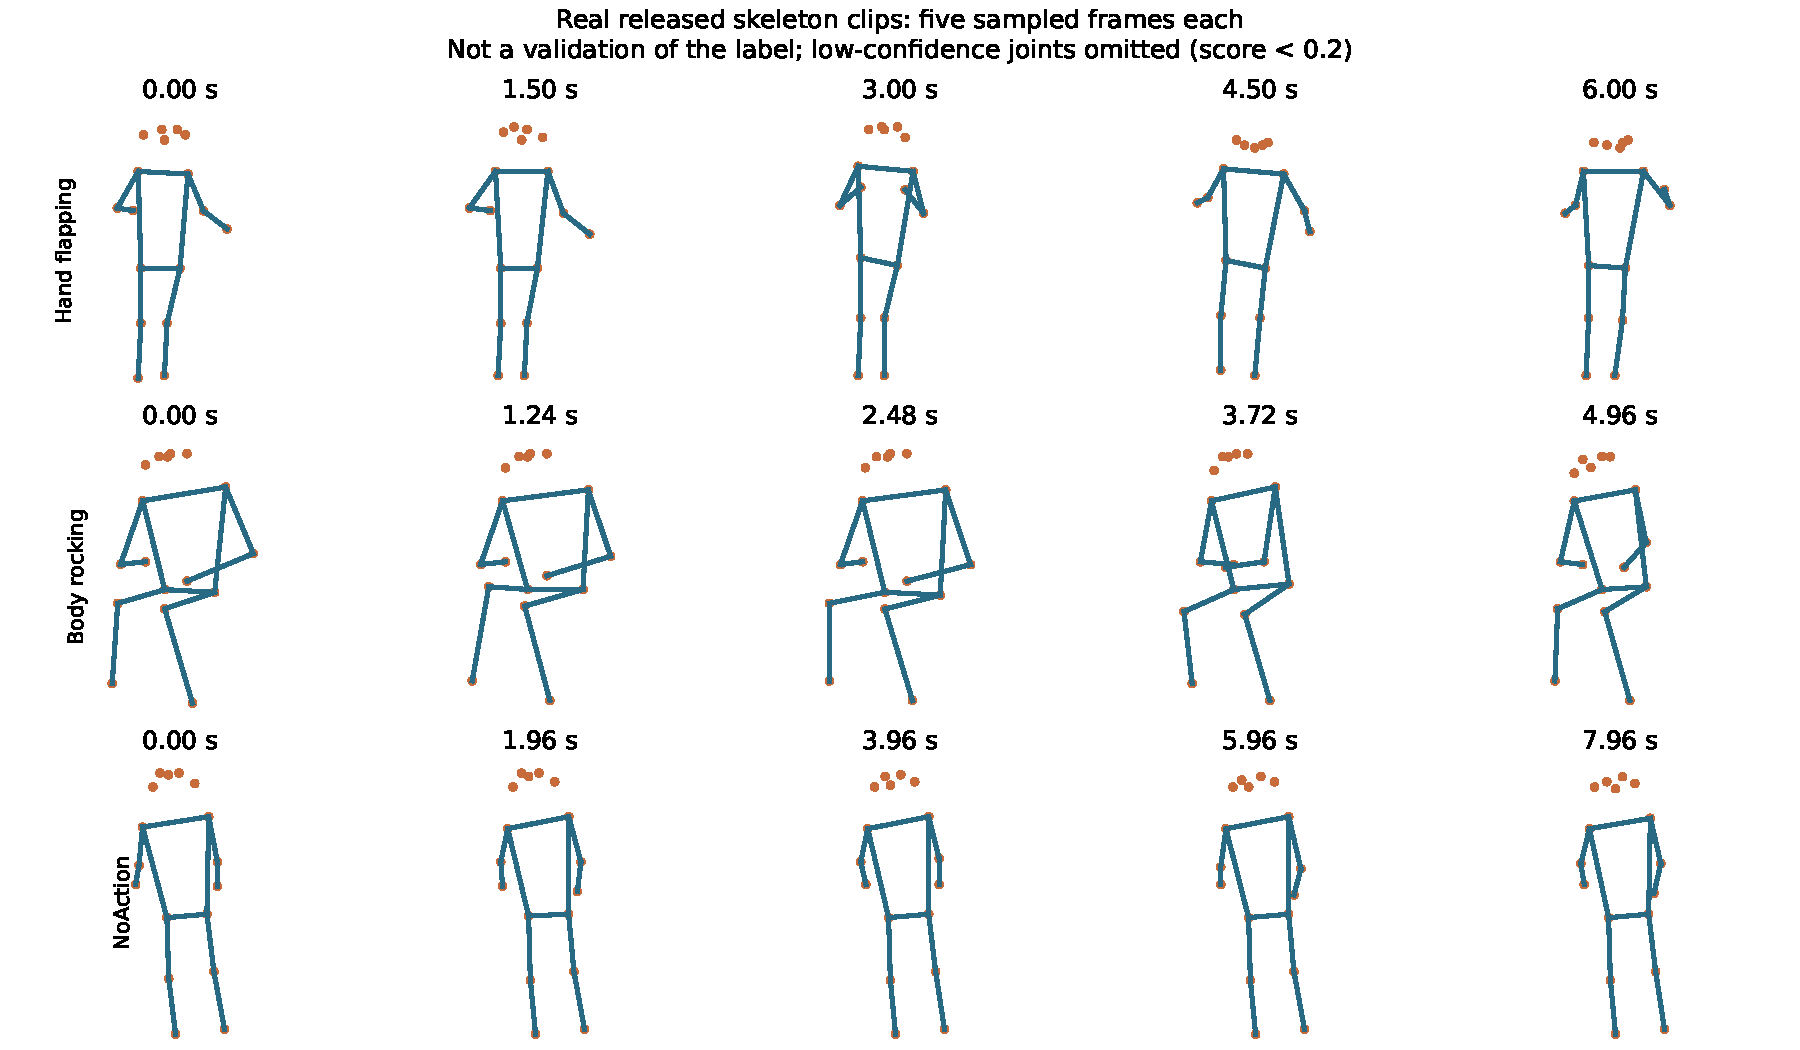
\includegraphics[width=\linewidth]{../../reports/figures/motion_examples.pdf}
\caption{Real skeleton examples selected for relatively good pose confidence, not randomly sampled representatives. Five frames cannot verify repetition or annotation correctness. Exact record identifiers and selection criteria are saved in \texttt{motion\_example\_manifest.json}.}
\end{figure}
\begin{figure}[p]\centering
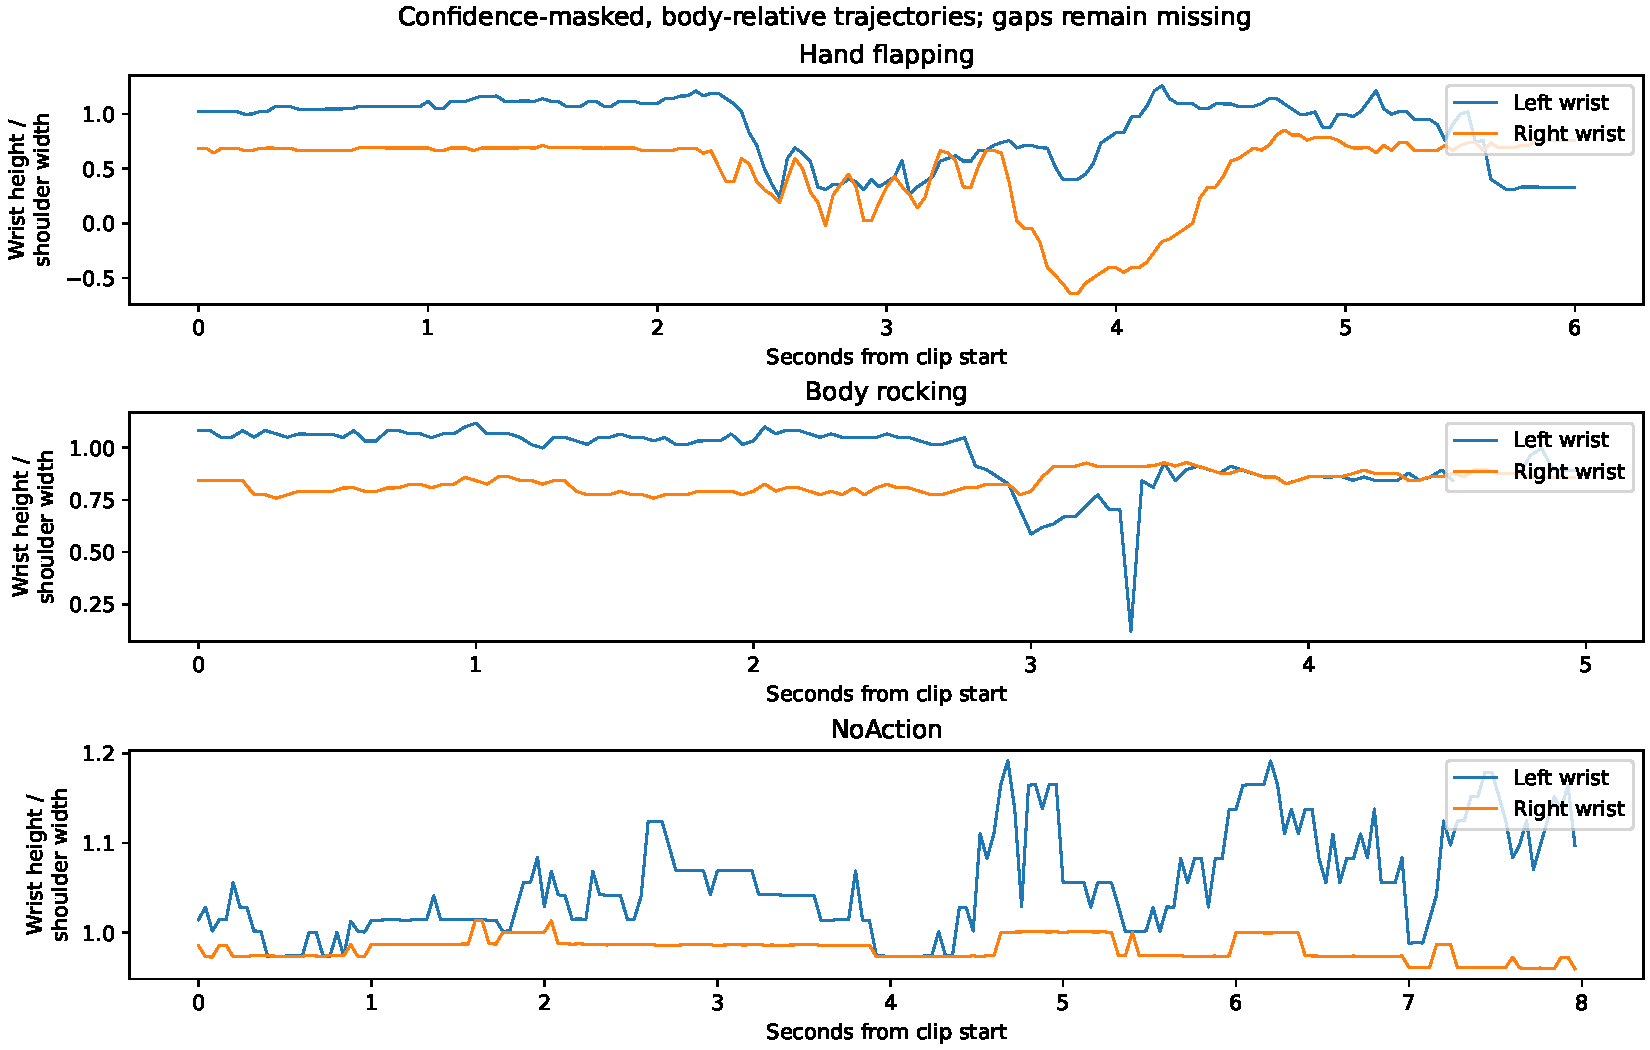
\includegraphics[width=\linewidth]{../../reports/figures/wrist_trajectories.pdf}
\caption{Body-relative wrist traces from the same clips. Missing points remain gaps. Smooth or periodic signals alone do not establish an SMM label; wrist-only features also miss lower-body and subtle finger movements.}
\end{figure}

\subsection{Repetition needs temporal structure, not only magnitude}
Let $x_t$ be one valid, regularly sampled scalar trajectory of $T$ samples, $\bar x$ its mean, and $\ell$ a lag in samples with $0\leq\ell<T$. On a contiguous valid interval with nonzero variance, normalized autocorrelation is
\[
R(\ell)=\frac{\sum_{t=1}^{T-\ell}(x_t-\bar x)(x_{t+\ell}-\bar x)}{\sum_{t=1}^{T}(x_t-\bar x)^2}.
\]
For a constant trajectory the zero denominator makes this normalized quantity undefined, not evidence of rhythmicity. Repeated peaks suggest recurrence; their time spacing is $\ell/f$. A spectrum or autocorrelation can summarize rhythm but is unreliable with few cycles, long missing runs or nonstationary motion. Interpolation through occlusions can manufacture smooth oscillations. Ordinary walking, clapping during a task and repetitive play can also be rhythmic, so periodicity is a candidate feature, not a definition of SMM.

Recurrence analysis instead asks when a trajectory returns to a similar state. Topological methods summarize the geometry of these returns. These may help explain repeated patterns without a large neural network; the recent MBaye study is discussed in the literature section. Whether they distinguish this release's heterogeneous positives from purposeful repetitive negatives is an experiment, not established transfer.

\subsection{Why PoseC3D uses heatmaps}
The source model turns each joint into a spatial confidence blob and stacks these across time. For heatmap pixel $(u,v)$, joint location $(x_{tj},y_{tj})$, confidence $c_{tj}$ and Gaussian width $\sigma$, an illustrative single-person joint heatmap is
\[
H_{tj}(u,v)=c_{tj}\exp\!\left[-\frac{(u-x_{tj})^2+(v-y_{tj})^2}{2\sigma^2}\right].
\]
Spatial convolution can tolerate small coordinate perturbations; temporal convolution learns changes in configuration. The three axes are image width, image height and time. They do not imply depth measurements. The source config uses 17 joint channels and 48 temporally sampled frames, with cropping, resizing and left/right-aware flips.\par
Sources: \artifact{resources/mmaction_template/binary_cfg_template.py}, pinned fork config, Supplement~1, pp.~7--8, and \href{https://openaccess.thecvf.com/content/CVPR2022/html/Duan_Revisiting_Skeleton-Based_Action_Recognition_CVPR_2022_paper.html}{Duan et al., CVPR 2022}, the original PoseC3D method paper archived locally.

This representation fits sparse body motion and avoids modeling appearance directly. It also inherits the pose extractor's failures: a missing wrist has no finger articulation, a wrong child remains wrong, and correlated confidence patterns can become shortcuts. Downsampling a 200-frame window to 48 samples also reduces temporal detail; the same 200 frames correspond to 8 seconds at 25 fps and 6.67 seconds at 30 fps. Equal frame counts are not equal physical durations.

\subsection{Algorithm choices as hypotheses}
\begin{longtable}{@{}P{.20\linewidth}P{.25\linewidth}P{.25\linewidth}P{.22\linewidth}@{}}\toprule
Method & Characteristic used & Why test it & What remains hard\\\midrule\endhead
Energy/angles + logistic model & Motion magnitude, joint geometry & Interpretable, cheap baseline; exposes whether complex models add value & Camera scale, task context and jitter\\
Autocorrelation, spectral or recurrence features & Repetition across time & Tests rhythmic structure beyond movement energy & Irregular bouts, few cycles, purposeful rhythms\\
Temporal convolution/LSTM & Sequential joint features & Learns order and duration with fewer spatial assumptions & Missingness, sampling rate, limited independent subjects\\
ST-GCN / adaptive graph model & Joint/bone relations through time & Explicit body connectivity; useful comparison to heatmaps & Graph depends on accurate joints; appearance/context absent\\
PoseC3D & Confidence-weighted space--time heatmaps & Published reference method and pretrained action representation & Compute, cropping, temporal resolution and quality shortcuts\\
Transformer or self-supervised encoder & Long-range dependencies or reusable motion structure & Later hypothesis when data quality and transfer protocol are stable & Many clips do not equal many independent children; pretraining leakage\\
Quality-aware multi-scale model & Visible-joint masks, multiple durations, uncertainty & Proposed main direction: reliability under heterogeneous missingness & Abstention can selectively exclude the hardest children\\\bottomrule
\end{longtable}
This table proposes a comparison program. It does not assert one model is superior on this release. The original alternative-model results are described separately in the paper section.

\subsection{From a clip score to an event and a session summary}
Let window $i$ cover the half-open frame interval $[a_i,b_i)$ and receive score $s_i$. For frame $t$ with one or more covering windows, the paper's aggregation is
\[
P_t=\max_{i:a_i\leq t<b_i}s_i,\qquad z_t=\mathbb{1}[P_t\geq\theta].
\]
Here $\theta$ is the classification threshold. Frames with no coverage must remain unknown. Taking the maximum means a single positive window raises every frame it covers; this tends to spread a decision over time and can merge neighboring events. Mean pooling, learned temporal localization or hysteresis could behave differently and require validation.\par
Source rule: \cite[p.~4]{barami2024}. Alternative choices are proposed experiments.

\begin{figure}[H]\centering
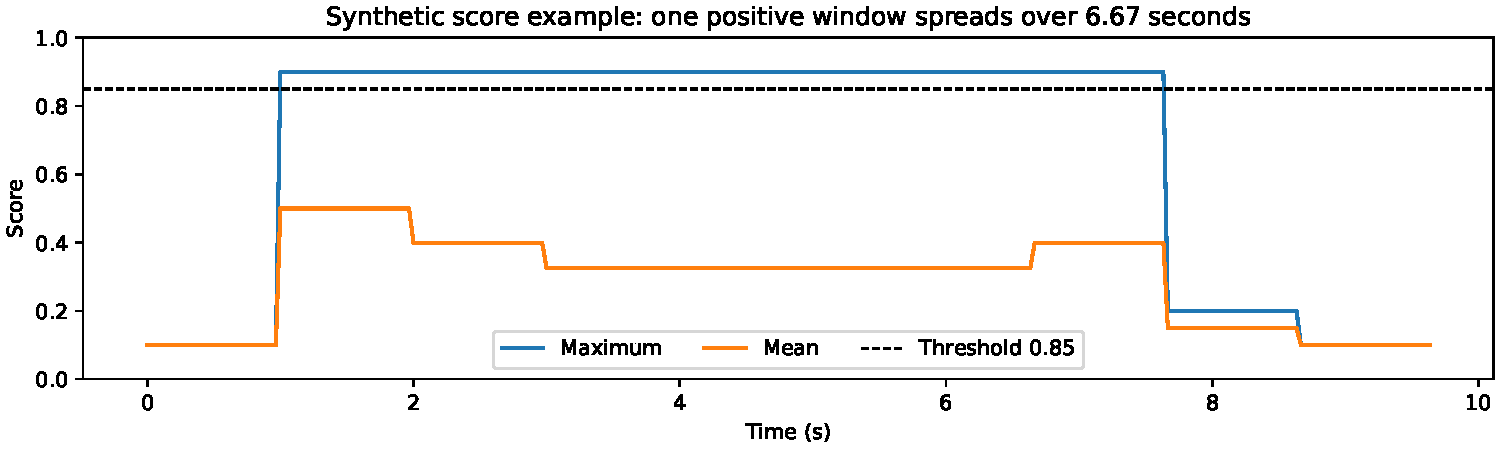
\includegraphics[width=\linewidth]{../../reports/figures/aggregation_demo.pdf}
\caption{Synthetic scores, not measured performance. Maximum and mean aggregation give very different frame decisions from the same windows. The final uncovered frames remain missing.}
\end{figure}

Let $\mathcal O$ contain frames where the child is observable under a predefined quality rule \emph{and} a finite covered prediction exists, and let $\Delta t=1/f$. Define detected time $D=\sum_{t\in\mathcal O}z_t\Delta t$ and observed-and-scored time $O=|\mathcal O|\Delta t$. Observable-and-scored burden is $B=D/O$ when $O>0$. Also report coverage $C=O/T_{\rm recording}$, where $T_{\rm recording}$ is the recording duration in seconds, and distinguish pose-visibility coverage from prediction coverage. A low-coverage recording cannot be treated as confidently low burden. Counting events requires an explicit rule for missing gaps, simultaneous camera views and minimum episode duration. A count per minute is $60N/O$ for event count $N$, with time measured in seconds.

\subsection{Evaluate the intended scientific claim}
\begin{description}[leftmargin=0pt]
\item[Clip discrimination:] precision--recall curves, per-class recall, calibration and quality-stratified errors. Clip accuracy is easily dominated by negatives or acquisition artifacts.
\item[Continuous event detection:] one-to-one episode matching at prespecified temporal intersection-over-union thresholds, onset/offset error, false events per hour and missed events. Frame accuracy alone can conceal clinically relevant errors.
\item[Burden measurement:] absolute and signed duration error, event-count error, agreement plots and observable-time coverage per child. A high correlation can coexist with systematic overestimation.
\item[Generalization:] group by verified child, preserve all sessions/views, tune only on training/validation, and bootstrap children as the independent unit. Site/camera/age/sex analyses require actual metadata and adequate numbers.
\end{description}
These are proposed evaluation requirements. The provided code currently executes release profiling, shortcut diagnostics, source counterexamples and visualization; it does not claim to have run this full predictive benchmark.

\clearpage
% Section fragment. Requires hyperref; no bibliography keys are used.
\section{Recent literature and research positioning}
\label{sec:literature}
\noindent Search cutoff: 16 September 2026. This focused scoping search covers the
original ASDPose release and nine complementary primary studies. The full search
log, source register, methodological qualifications, and download manifest are
preserved in \texttt{reports/literature\_survey.md} and
\texttt{references/papers/literature\_downloads.json}.

\subsection{Has the released dataset been reused?}
No independent reuse of the released ASDPose files was verified in this search.
This is a bounded retrieval result, not evidence that no reuse exists. Exact
ASDMotion/ASDPose searches and citation-neighborhood searches found relevant
studies with different cohorts. For example, Freud et al. and Amraee et al. cite
Barami but describe separate experiments. Shared authors or an ADOS assessment
context do not establish identical data. The original release remains the direct
baseline: \href{https://doi.org/10.1001/jamanetworkopen.2024.32851}{Barami et al.,
JAMA Network Open, 2024}.

\subsection{Different questions require different observations}
\begin{description}
\item[Repetition structure.]
\href{https://doi.org/10.1038/s41598-026-60095-8}{MBaye et al., Scientific Reports,
July 2026} construct interpretable persistent-homology features. The publisher
identifies an accepted early article; detailed methods in our review refer to
the \href{https://doi.org/10.1101/2025.09.03.674008}{September 2025 preprint}.
It uses a distinct six-participant video/accelerometer cohort. Periodicity is
a useful candidate representation, not demonstrated ASDPose transfer.

\item[Concurrent movement categories.]
\href{https://doi.org/10.1002/aur.70020}{Lemler et al., Autism Research, March 2025}
use OpenPose and an LSTM for multi-label flapping/jumping recognition. With
subject-disjoint nested validation, macro accuracy is 0.702 but macro F1 is
0.318. This study makes performance under new-child evaluation especially
important; its Frankfurt cohort is separate.

\item[Multimodal action recognition.]
\href{https://doi.org/10.1109/JBHI.2024.3511601}{Zhang et al., IEEE JBHI,
March 2025 issue} combine RGB, optical flow, and skeletal structure with APMFNet
on ACSA653. Such fusion requires modalities that cannot be recovered from a
body-skeleton release. The author manuscript is archived locally for protocol
comparison.

\item[Interpersonal coordination.]
\href{https://doi.org/10.1038/s41598-024-56098-y}{Koehler et al., Scientific
Reports, March 2024} classify patient--clinician dyads from motion synchrony.
Balanced accuracy is 63.4\% against clinical controls. The authors discuss the
possible influence of clinician movement. This is a dyadic clinical-comparison
question rather than SMM episode detection.

\item[Neural mechanisms of imitation.]
\href{https://doi.org/10.1038/s41597-025-05313-0}{Paulo et al., Scientific Data,
June 2025} introduce Move4AS: EEG with marker-based 3D motion during walking
and dancing imitation. It enables neural--motor questions requiring different
sensors and an experimental task.

\item[Purposeful fine motor control.]
\href{https://doi.org/10.1002/aur.70049}{Freud et al., Autism Research, May 2025}
analyze thumb/index-finger grasping in young adults, obtaining over 84\%
classification accuracy with subject-wise validation. The population and
fine-grained measurement differ from preschool body-pose video. Their result
does not validate diagnosis from ASDPose.

\item[Measurement agreement and facial context.]
\href{https://doi.org/10.1186/s13229-025-00685-x}{Manelis-Baram et al., Molecular
Autism, October 2025} compare three facial-expression tools. Outputs differ,
but expression quantity does not significantly distinguish groups. The study
leaves timing, quality, and social context unresolved and is not verified reuse
of the released skeleton data.

\item[Event-level kinematics.]
\href{https://doi.org/10.1111/desc.70176}{Stenum et al., Developmental Science,
March 2026 online} find that event-level amplitude differences disappear after
averaging. This separate toddler cohort cites Barami but does not reuse ASDPose.
Data access requires author request and a data-use agreement.

\item[Semantic behavior context.]
\href{https://openaccess.thecvf.com/content/CVPR2026W/CV4Smalls/papers/Amraee_Toward_Automated_Behavior_Understanding_in_Autism_A_Zero-Shot_Vision-Language_Model_CVPRW_2026_paper.pdf}{Amraee
et al., CVPR Workshops, June 2026} classify 40 clips with vision-language
descriptions and prompted language models. The target includes self-injury,
aggression, and property destruction. This requires visual context and is a
small separate evaluation, not ASDPose benchmarking.
\end{description}

\subsection{Proposed research direction: trustworthy motion measurement}
The following proposals are our synthesis, not results reported by the cited
studies. A useful first research question is:
\begin{quote}
How reliably can SMM burden be estimated for unseen children when pose quality,
missing intervals, and temporal uncertainty are explicitly represented?
\end{quote}
This question has a data-availability gate. The inspected training release
contains 36,930 clips; it does not establish a complete recording timeline or
continuous annotation coverage. Boundary units, source-recording correspondence,
and participant mapping require confirmation. Consequently, clip-level
measurement reliability is the directly feasible first stage. Full-session
burden evaluation must wait for validated continuous recordings, complete event
intervals, and an observed-time denominator. These are local audit findings,
documented in \texttt{data/processed/dataset\_summary.json},
\texttt{dataset\_structure.json}, and \texttt{eda\_notes.json}; the continuous
archive was pending at this review stage. The proposed sequence is:
\begin{enumerate}
\item Freeze participant-disjoint splits before choosing features or thresholds.
Verify interval units and continuous label coverage before estimating burden.
Summarize recording length, repeated sessions, visible-body coverage, joint
confidence, missing runs, and track discontinuities.
\item Establish simple motion-energy and periodicity baselines. Compare
autocorrelation/spectral features with recurrence or topological features before
claiming benefits from a more complex representation.
\item Reproduce the original temporal labeling and inference rules. Report all
deviations between paper, repository, and available release.
\item Compare confidence-aware features or masking and multiple temporal scales
with the same baseline, children, labels, and evaluation procedure.
\item Evaluate precision--recall, episode matching, false events per hour, and
duration/burden error. Bootstrap children, not overlapping windows. Tune
calibration and thresholds on validation data only.
\item Explore clinical associations only after reliability is demonstrated.
Handle repeated sessions and prespecify covariates; do not interpret association
as a causal mechanism or treatment response.
\end{enumerate}

\paragraph{Tests that could disprove the proposed benefit.}
An uncertainty-aware method is not useful merely because its aggregate score
improves. Check whether the improvement persists at matched recall, in children
with fewer visible joints, and after matching movement energy. Test ordinary
periodic activity, track jumps, weak/aperiodic events, overlapping people, and
short bouts as separate error strata. Report abstention coverage and the share
of time that cannot be measured. Negative results are informative if they expose
a representation limit.

\paragraph{Proposed event-distribution analysis.}
Motivated by Stenum's distinction between events and averages, compare
within-child distributions of wrist/body amplitude and recurrence instead of
only a single child mean. This is our proposed experiment, not a published
ASDPose result. The release includes subtype and combined action strings, which
need an ontology and concurrency audit. A label such as ``Fingers'' does not
provide finger coordinates in the observed 17-joint body representation.

\paragraph{Questions requiring additional data.}
Diagnostic discrimination needs an appropriate non-ASD clinical comparison
cohort. Subtype discovery needs trustworthy subtype annotation or careful
external validation of clusters. Social synchrony needs stable partner identity
and role. Facial expression, semantic object interaction, EEG coupling, and
finger-level grasping require modalities beyond the released body coordinates.
Longitudinal treatment claims require intervention and follow-up information,
not just repeated recordings.

\paragraph{Reading order and durable evidence.}
Read the original methods with the local schema audit first, then Lemler for
evaluation design and MBaye for interpretable recurrence. Read Koehler and
Manelis-Baram to examine context and measurement validity. Use Move4AS, grasping,
multimodal fusion, and VLM work when choosing whether a later research question
justifies additional data. Citation counts were not reliably refreshed and are
not used to rank evidence. Publisher/author URLs, affiliations, dates, access
failures, and paper hashes are recorded in the Markdown report and manifests.

\clearpage
\section{Phased research plan and decision gates}\label{sec:plan}
\subsection{Phase 0: establish exactly which data exist --- completed}
Downloaded source, labeled clips, continuous skeleton archive and checkpoint; archived the paper, supplements and accessible related work; preserved hashes, commit records and access limitations. Deliverables are the raw manifest and source register. The archive includes an explicit child/assessment/camera table; its relationship to the labeled file still needs validation. Do not overwrite these originals during experimentation.

\subsection{Phase 1: understand the release and measurement process --- completed}
Profiled all 36,930 labeled records, their shape, labels, confidence, frame rate, duration, duplicates and release split. Created real skeleton/trajectory examples. Inspected continuous skeletons and their metadata separately. Audited source code with executable counterexamples. The key result is that metadata and missingness can provide strong label cues, so a clip-classification score alone will not establish useful motion recognition.

\subsection{Phase 2: reconstruct an auditable dataset --- specified, mapping unresolved}
The next action is a precise release-reconciliation request, drafted in \artifact{docs/OPEN_QUESTIONS.md}; no message was sent. Needed answers: labeled-file version, participant crosswalk, original split, units/padding of boundaries, 25/30-fps processing history, whether negative labels exhaustively cover the continuous archive, and zero-pose policy. Meanwhile, retain every original field and use a unique internal \artifact{record_index}; do not deduplicate by identifier alone.

After the mapping is verified, create a canonical manifest with participant, assessment, camera, clip, original timing, fps, preprocessing version, label provenance and quality coverage. The provided \artifact{scripts/03_make_grouped_splits.py} enforces complete explicit mapping and blocks subject or nonzero exact-coordinate overlap between partitions. All-zero hash collisions are audited as missing-data patterns. It deliberately does not infer subjects from filename tokens. Adapt the released clip schema to MMAction2 only after confirming label direction and the correct child axis. Maintain an untouched test set and a distinct validation set.

\textbf{Gate:} no claim of subject-independent performance until identities are established; no continuous burden claim until full event coverage and timing are aligned. Removing bad clips can alter the population. Report the number removed by child and label and preserve a documented unusable-data stratum.

\subsection{Phase 3: measure simple baselines before selecting architecture}
First compare metadata-only, quality-only, motion-energy, body-relative angle/velocity and periodicity baselines. Metadata-only models are diagnostic controls; they are not the intended research model. The present fps-only rule is post-hoc descriptive evidence and should not be presented as a competitive score.

Within a verified split, test duration-matched, fps-matched and quality-matched subsets with their original unfiltered counterparts. The 25-fps subset contains both classes and is a useful sensitivity analysis, but it changes the positive population; there is no 30-fps negative comparison in the current release. Re-extraction from a uniform source pipeline would be stronger if the required source material becomes available. Report the sample and participant loss from every restriction.

\textbf{Gate:} if performance largely disappears after controlling acquisition, investigate data construction before architecture. If an interpretable motion baseline remains informative, identify its systematic failures before adding a neural model.

\subsection{Phase 4: reproduce and then improve recognition}
Repair the confirmed code defects in an isolated fork with tests. Reproduce the paper's representation, model and temporal processing under a documented compatible environment, while explicitly labeling unresolved historical hyperparameters and dataset differences. A modern rerun is not an exact reproduction merely because it uses PoseC3D.

Proposed experiment ladder: (A) body-relative features; (B) ST-GCN/temporal model; (C) PoseC3D reference; (D) confidence-masked or uncertainty-aware variant; (E) multi-scale temporal variant. Keep children, quality policy, supervision, optimization budget and evaluation constant where possible. Factorial ablations should separate the benefits of representation, extra context, confidence handling and temporal aggregation. Do not attribute a gain to a new network when it came from cleaning labels or changing data selection.

\subsection{Phase 5: temporal localization and full-session burden}
Conditional on validated continuous labels, compare max pooling with mean/hysteresis/localization alternatives. Use event, frame and burden metrics simultaneously. Evaluate short bouts, long bouts, missing joints, camera changes, ordinary periodic play and transitions. Quantify onset/offset uncertainty and observation coverage. Multi-camera fusion requires synchronization and an explicit rule to avoid counting the same event twice.

The clinically meaningful output is a behavior measurement with uncertainty and coverage, not an assertion that every detected repetitive movement is harmful. SMMs may be self-regulatory; the dataset does not reveal subjective function or treatment need. \cite[pp.~2--3]{barami2024}

\subsection{Phase 6: broader ASD questions require new evidence}
\begin{longtable}{@{}P{.27\linewidth}P{.32\linewidth}P{.33\linewidth}@{}}\toprule
Research question & What current data can contribute & Additional requirement\\\midrule\endhead
Robust SMM recognition & Labeled body-motion clips and confidence & Resolved mapping, confound controls and verified split\\
Subtype description & Atomic and combined movement labels & Label reliability, enough independent examples, sensitivity to incomplete body representation\\
Fine finger or facial behavior & Coarse wrist/head proxy only & Hand/face landmarks or authorized raw video; validate extraction\\
ASD diagnosis/screening & A positive-cohort representation to investigate & Non-ASD and other developmental controls, prospective design and external validation\\
Social synchrony & Possibly a future methodological component & Stable partner tracks and roles; present child-only release is insufficient\\
Clinical severity/development & Candidate reliable motor measurements & Linked clinical/demographic scores and repeated-session design\\
Treatment effects or causality & Baseline measurement methodology & Intervention assignment, follow-up and causal design; cross-sectional association is insufficient\\
Neural mechanisms & Motion features as a potential modality & Synchronized EEG/other physiology and experimental conditions\\\bottomrule
\end{longtable}

\subsection{Recommended initial research direction}
\textbf{Working question: Can heterogeneous SMMs be recognized from 2D skeletons in a way that remains valid across pose quality and acquisition conditions?} This is a proposed direction, not a claimed novelty statement. Its first contribution would be a transparent dataset/protocol audit; its modeling contribution would need to demonstrate improvement under verified child-disjoint and confound-controlled evaluation.

A concrete null hypothesis is that confidence-aware or periodicity-aware modeling adds no benefit beyond simple motion features after controlling acquisition artifacts. Rejecting that null requires matched evaluation and confidence intervals at the child level. If it is not rejected, the useful finding may be a representation or annotation limit. Full-session burden is the next stage once continuous labels and mapping become trustworthy. A larger transformer is not the first unresolved scientific question.

\subsection{Hard limits versus problems that can be engineered}
Code failures, inconsistent schema, event merging and missingness accounting are repairable engineering problems. Acquiring a verified participant crosswalk, original label provenance and a consistent extraction history requires information from the data producers. Inferring finger motion, emotional function, ASD specificity or causal treatment effects from child body coordinates alone is an information limitation; changing architecture cannot create absent observations. Domain shift to homes, different ages or clinical populations requires new evaluation data, even if within-release accuracy is excellent.

\subsection{Durable working practice}
Read \artifact{README.md}, \artifact{docs/PROJECT_STATE.md} and \artifact{docs/OPEN_QUESTIONS.md} before continuing. Each experiment must record the raw-data hashes, split-manifest hash, code revision, environment, seeds, preprocessing policy, training/selection budget and metric definitions. Save failed experiments and reasons. The project state distinguishes completed analysis from future plans; no step relies on conversational memory.

\clearpage
\section{Provenance, reproducibility and limits}
The main repository was downloaded as a source ZIP because the local Git HTTPS helper was unavailable. The GitHub commit API identifies \artifact{f699dc7b7af5726df5d8e79161d192eac22cfafb} (3 October 2025); the ZIP and unmodified source are retained. Fork snapshots and their commit record are stored in \artifact{references/source_snapshots/}. Raw data checksums are local integrity anchors, not author-supplied authenticity signatures. All three repository-linked files were downloaded. The checkpoint is preserved but was not deserialized or run.

The labeled clip audit covers every record. All 914 continuous skeleton files were also profiled; the scope and results are in \artifact{data/processed/continuous_summary.json}. Metadata and array checks do not visually validate every trajectory's child identity. The study paper, both supplements, and several accessible related PDFs are archived. Source and download manifests record retrieval limitations. Citation counts were not reliably available and were not invented. The literature search is a focused scoping review through 16 September 2026, not a preregistered systematic review.

No GPU training, full historical-model reproduction, raw RGB re-extraction, ASD diagnosis experiment, or clinical subgroup association is claimed. Training requires a validated split and compatible model environment. The modern CPU analysis environment is intentionally separate from the historical Python 3.9/PyTorch 1.13/MMAction2 stack.

\textbf{Audit record.} Product: Codex desktop; execution location: Local, Windows. Capabilities used: shell/Python, public-web retrieval, NumPy/Pandas data inspection, PDF extraction, LaTeX, parallel independent source and code audits. Effective source-audit mode: parallel-subagents; main author reconciled results against local artifacts. Numerical descriptions of downloaded data are generated by code. Own proposals are labeled as proposals. Paper figures are original-page extracts, never reconstructed as if they were the original.

\begin{thebibliography}{9}
\bibitem[Barami et al., 2024]{barami2024} T. Barami, L. Manelis-Baram, H. Kaiser, et al. Automated Analysis of Stereotypical Movements in Videos of Children With Autism Spectrum Disorder. \emph{JAMA Network Open}, 7(9):e2432851, 12 September 2024. \href{https://doi.org/10.1001/jamanetworkopen.2024.32851}{doi:10.1001/jamanetworkopen.2024.32851}. Open access, CC BY. Main paper and Supplements 1--2 are archived locally.
\bibitem[Dinstein Lab, 2025 snapshot]{repo} Dinstein-Lab. ASDMotion source repository. Snapshot commit f699dc7, last commit 3 October 2025, retrieved 16 September 2026. \url{https://github.com/Dinstein-Lab/ASDMotion}. MIT code license. Dataset access statement is separate from code licensing.
\end{thebibliography}
\end{document}
